\section{くまのせいかつとその他もろもろ}\label{sec:kumanoseikatu}

\bunsekisha{文責}{午後三時}

\subsection{まえがき}
これから熊野寮に入寮するかもって思った人に、ちょっとでも雰囲気とか伝わったらいいなと思って。まだ入寮して1年もたってないけれど一応私が思ったこととかなんとか。

\subsection{寮食について}
\begin{wrapfigure}[8]{r}[1cm]{4cm}
  \centering
  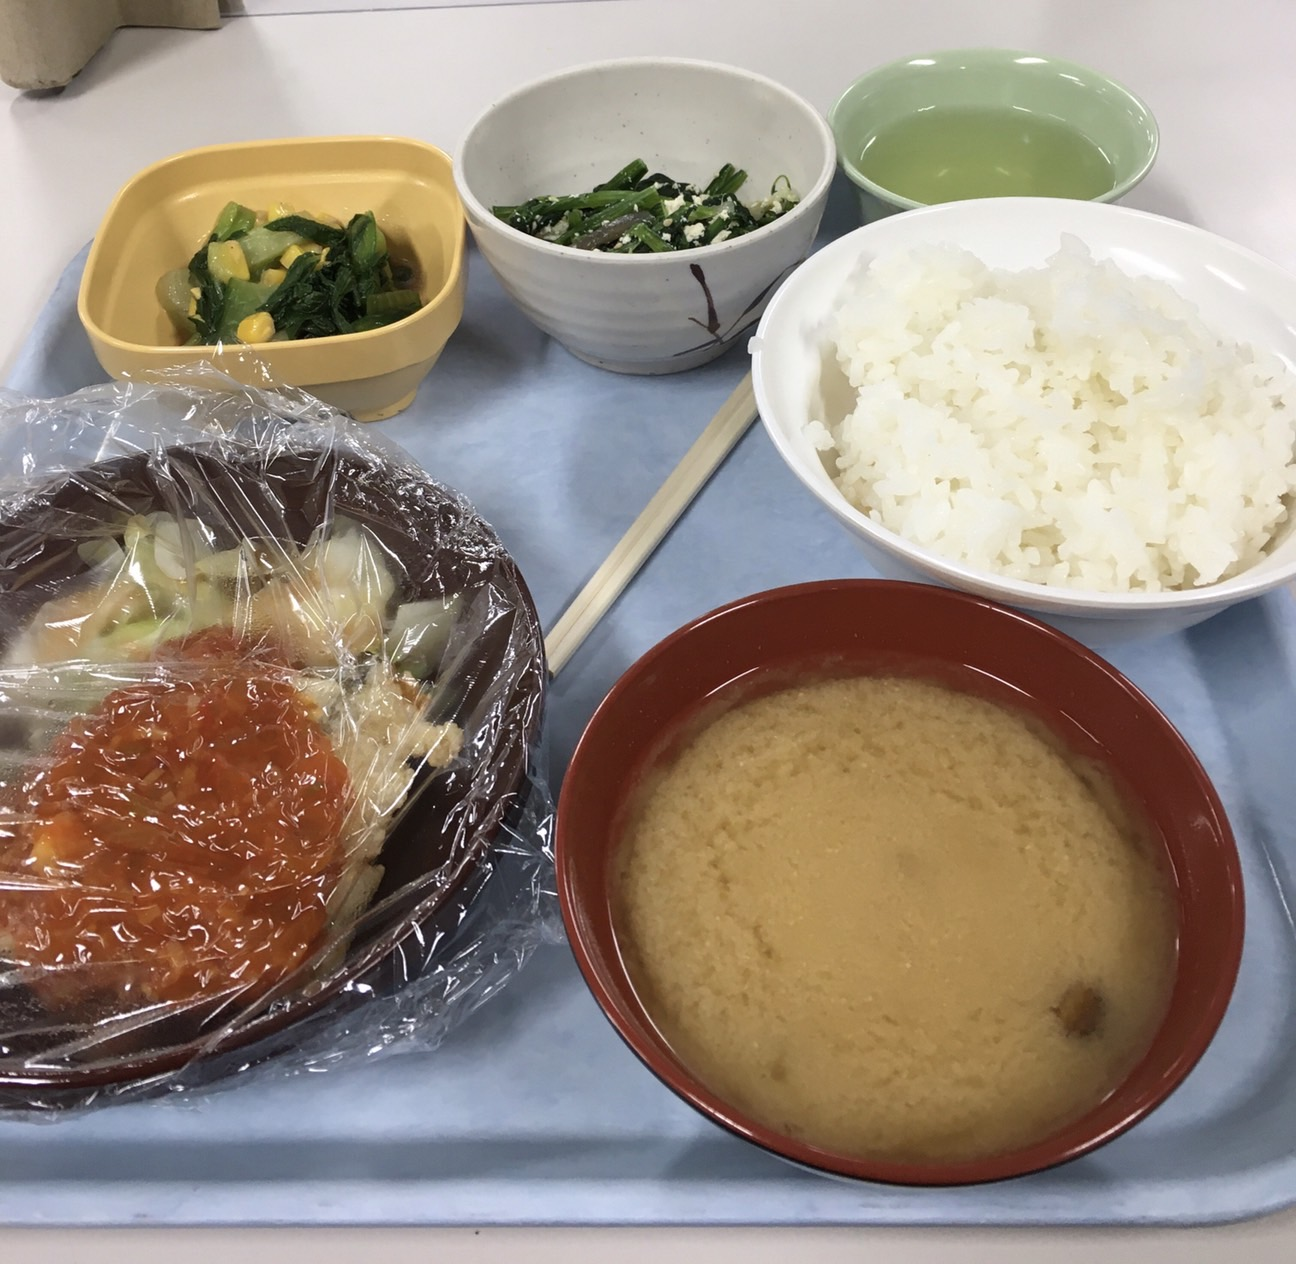
\includegraphics[width=3.8cm]{gazo/hanbagu.jpg}
\end{wrapfigure}

% \begin{floatingfigure}{5cm}
%   \centering
%   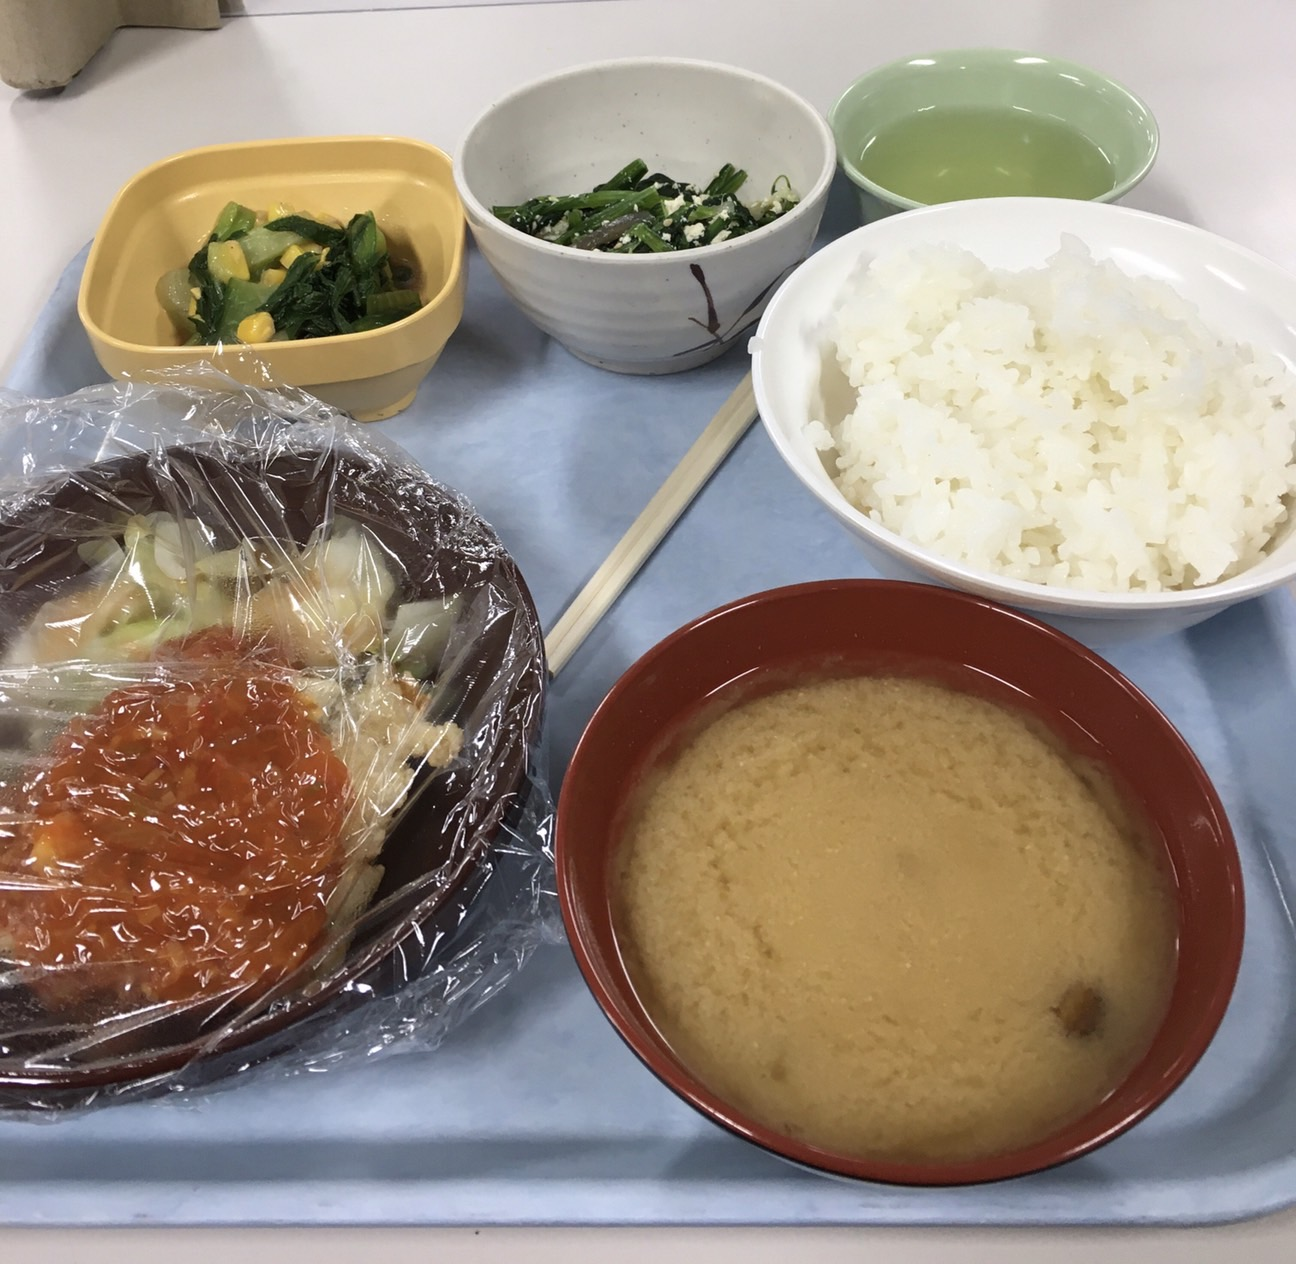
\includegraphics[width=4.8cm]{gazo/hanbagu.jpg}
% \end{floatingfigure}


寮食はおいしい。そして自分で作らなくてよくて帰ったらすぐに食べられてお皿も当番の人が洗ってくれて量が多くて安いのが本当に素晴らしい。特に今は冬なので温かいご飯が待っているという幸せを毎日のようにかみしめている。私は好き嫌いが多いうえにあんまり料理ができないので、完全に食事つきだと困る、でも完全に自炊もしんどそうという状況で、(食堂防衛的に食べたほうがいいのはもちろんだが)食券制で苦手なメニューの時は食べなくてもよい寮食はぴったりの制度だった。喫食時間が決まっているものの残置(前日や当日に寮食を予約しておくみたいな制度)等をすれば困るような時間ではない。ちなみに昼寮食ならタコライス、二色メニューの時はご飯派、夜寮食はタラとかの白身魚のフライと香草焼きが好きです。入寮した暁には寮食を食べよう!入寮しなくても熊野寮生と友達になれば一緒に食べられるので、入寮しなくても是非食べてほしい。



\subsection{シャワー、トイレについて}
去年までピカピカの予備校に住んでいたみたいな人がみて、おおーきれい!となるようなきれいさではない。が、ものすごく汚いわけではない。きれい(熊野比)というかんじ。でも少なくとも住むうえでネックになることはよっぽどないと思う。たまに水漏れしたりとかはあるが、一応ちゃんと直してくれる。個人的には、水回りの掃除を清掃員の方がやってくれて自分でほぼやらなくていいというのが地味に大きな助かるポイントだと思っている。

\subsection{部屋について}
A、B棟が基本4人部屋なのに対し、私が住んでいるC棟は基本2人部屋、しかも人数の関係で2部屋を1部屋寝室1部屋リビングとして3人で使うというだいぶイレギュラーな感じなので参考になるかはわからない。そもそも部屋なんてたぶん同じブロック内でもだいぶ違うと思う。とりあえず私の部屋はこんな感じということを。

前の住人の方が家具を残し私物を持っていき、たぶん頑張って掃除をしてくれたおかげで引っ越してから大きなものを買い足す必要はほぼなかった(部屋によっては前の人の靴下とかが出てきたとかなんとか)。ただ当時は両部屋とも土足で使っていたっぽく、寝室のほうは床がコンクリのままだった。その後、同部屋の方がとてもキレイに掃除してくださったうえ、同部屋の3人で割り勘して床材を買ってフローリングにしてなんかいい感じになった。床がフローリングだと座れて使えるスペースも増えるし、ぱっと見て普通の部屋という感じが出てびっくりした。冷暖房器具としては寝室にはエアコンがあってリビングには電気ストーブがあった。どちらもどうせ壊れてるだろうと思っていたらちゃんと使えた。ただみんながみんなMAXで冷暖房器具を使うと一瞬にしてブレーカーが落ちるので、談話室とか食堂であつまって温まろうという話はある。個人的な感覚としては夏の食堂はどうしようもなく暑いけど、冬の食堂はそこそこ暖かい気がする。虫とかは今のところそんなに見てない。小学校の教室くらい?1階だったり民青池の近くだったりすると多くなるかもと言われてはいる。たぶん入寮時の用紙に虫は平気かみたいな質問があった気がするから、そこに苦手と書いておけば考慮してくれるかも。プライバシーとか一人の時間は、うちは2部屋あるからというのもあるけど全くないということはないと思う。同部屋の方が2人とも授業やサークル、談話室などに行っていて部屋にひとりという時間は意外とある。あとは部屋に入る前にノックをしようとか、就寝時間が違うのでベッド周りはカーテンなどで仕切りを作るとかということをしていただいています。

\subsection{談話室について}
具体的に何があるかはC12談話室大解剖のページを参照(p.\pageref{daikaibo_danwa})。ほかの談話室のことはあんまり知らない。C34談話室は漫画がいっぱいある。あとこたつが何個もあるのとヨギボーがあるのはうらやましいかも。ここでは機能的精神的談話室の話を。

私が一番好きなのは深夜3時とか4時とかに2、3人くらいでゆったりぼーっとしながら、こたつに入ったり椅子にもたれたりしてとりとめもない話をする時間。自分がそもそも一人でいても生活習慣乱れがちな人で、眠たいときは9時とかに寝るし眠れないときは3時を過ぎても眠れないので、そういうときに話せる誰かがいてくれるのは本当にありがたい。あとは麻雀したりゲームしたり、ゆるっとした飲み会したり、ごはんを一緒に食べたり一人じゃなかなかできない楽しいことができるのがとても良いです。勉強はやろうとはするけど、結局談話室ではあんまりはかどらないことが多い。朝6時7時くらいならあんまり人がいなくてはかどるらしい。

寮の設備についてはホームページの動画から雰囲気が伝わると思います。\\
「京都大学熊野寮 施設紹介」\url{https://youtu.be/pcP7SKIyyxk} - YouTube

\subsection{コンパについて}
特に新歓期はたくさんコンパがあるけれど、コンパに絶対に参加しないといけないとか無理やりお酒を飲まされるとかはないので心配しなくていい。むしろ適量がわからないまま飲みすぎたときに、ストップをかけてくれたり介抱してくれたりする周りの人がいることはいいと思う。迷惑をかけないにこしたことはないけれど。上下関係もないことはないんだけど、むしろ1回生や新入寮生を大事にしてくれる雰囲気があると思います。いろんな人と話せて楽しいし、引っ越したばかりの時に夕食1食分くらい食べられるのはありがたかった。

\subsection{屋上について}
\begin{wrapfigure}[8]{r}[1cm]{5cm}
  \centering
  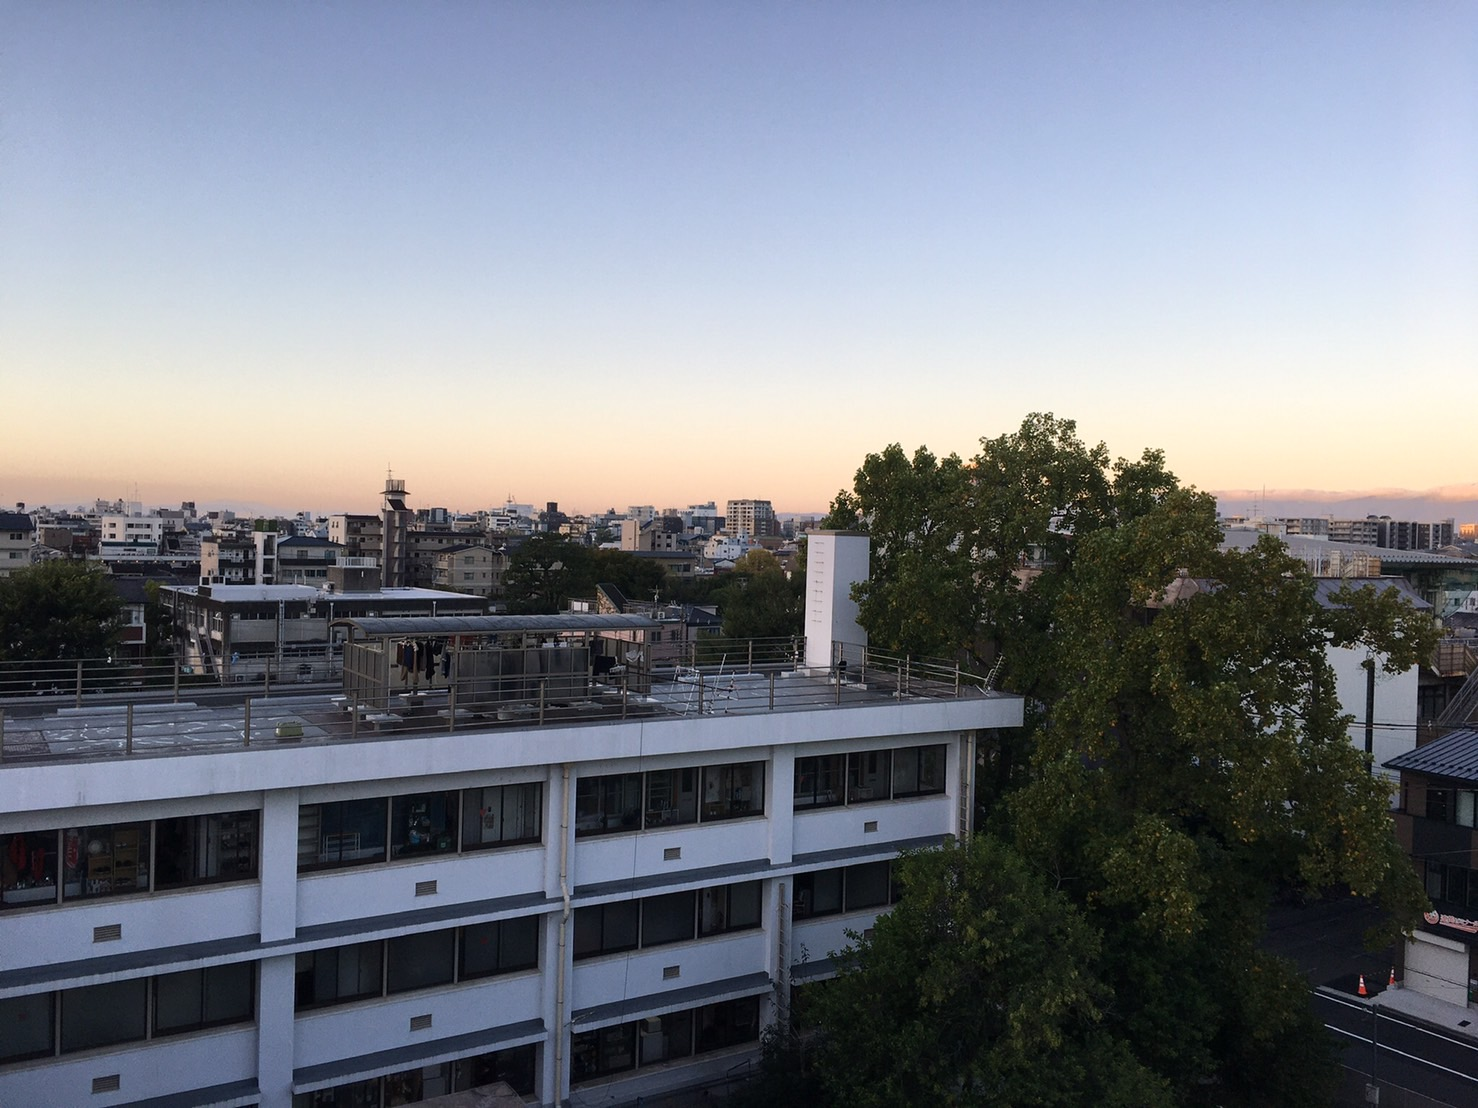
\includegraphics[width=4.8cm]{gazo/okujo.jpg}
\end{wrapfigure}


個人的に寮内で一番好きな場所。コンパとかでたくさんの人に会ってちょっと疲れたなってときに屋上に行くと、食堂の喧騒を遠くに聞きながら一人になって落ち着く。夕焼けもきれいだし、大文字山も見える。朝もまた朝焼けを見たり、向かいのパン屋さんや和菓子屋さんのの開店を見たりできる。バスを待っている人や丸太町通りの横断歩道以外のところをなんとか横断しようとする人、寮を見上げる観光客などいろんな人を見ることができる。最高。%\zenkakuspace{200}

\subsection{寮外のおすすめスポットについて}
独断と偏見によって適当に選んだ。他にもいいところはたくさんあるけれど、せっかくなので半分はちょっとニッチなところを。

\subsubsection{鴨川}
言わずと知れたいいところ。東大と京大ちょっと迷ってるみたいな話を聞いたときに、大学については自分は何とも言えないけれど、生活の中に鴨川があるかないかでは全然違うよ!と力説してしまった。鴨川沿いを自転車で走る時間は春夏秋冬ずっと好きだった。自分にとって大切な時間の隣にずっと鴨川があった気がする。

\subsubsection{大文字山}
こちらも有名どころ。意外と簡単に登れて、火床から京都の町が一望できる。ぜひ大文字コンパにも参加してね。個人的おすすめは平日の夕方、空が水色からピンクに変わりはじめた時間帯。日の入りや夜景を見るのもいいし、日中に行って自分の知っている場所を探すのも楽しい。

\subsubsection{宝ヶ池}
\begin{wrapfigure}[8]{r}[1cm]{5cm}
  \centering
  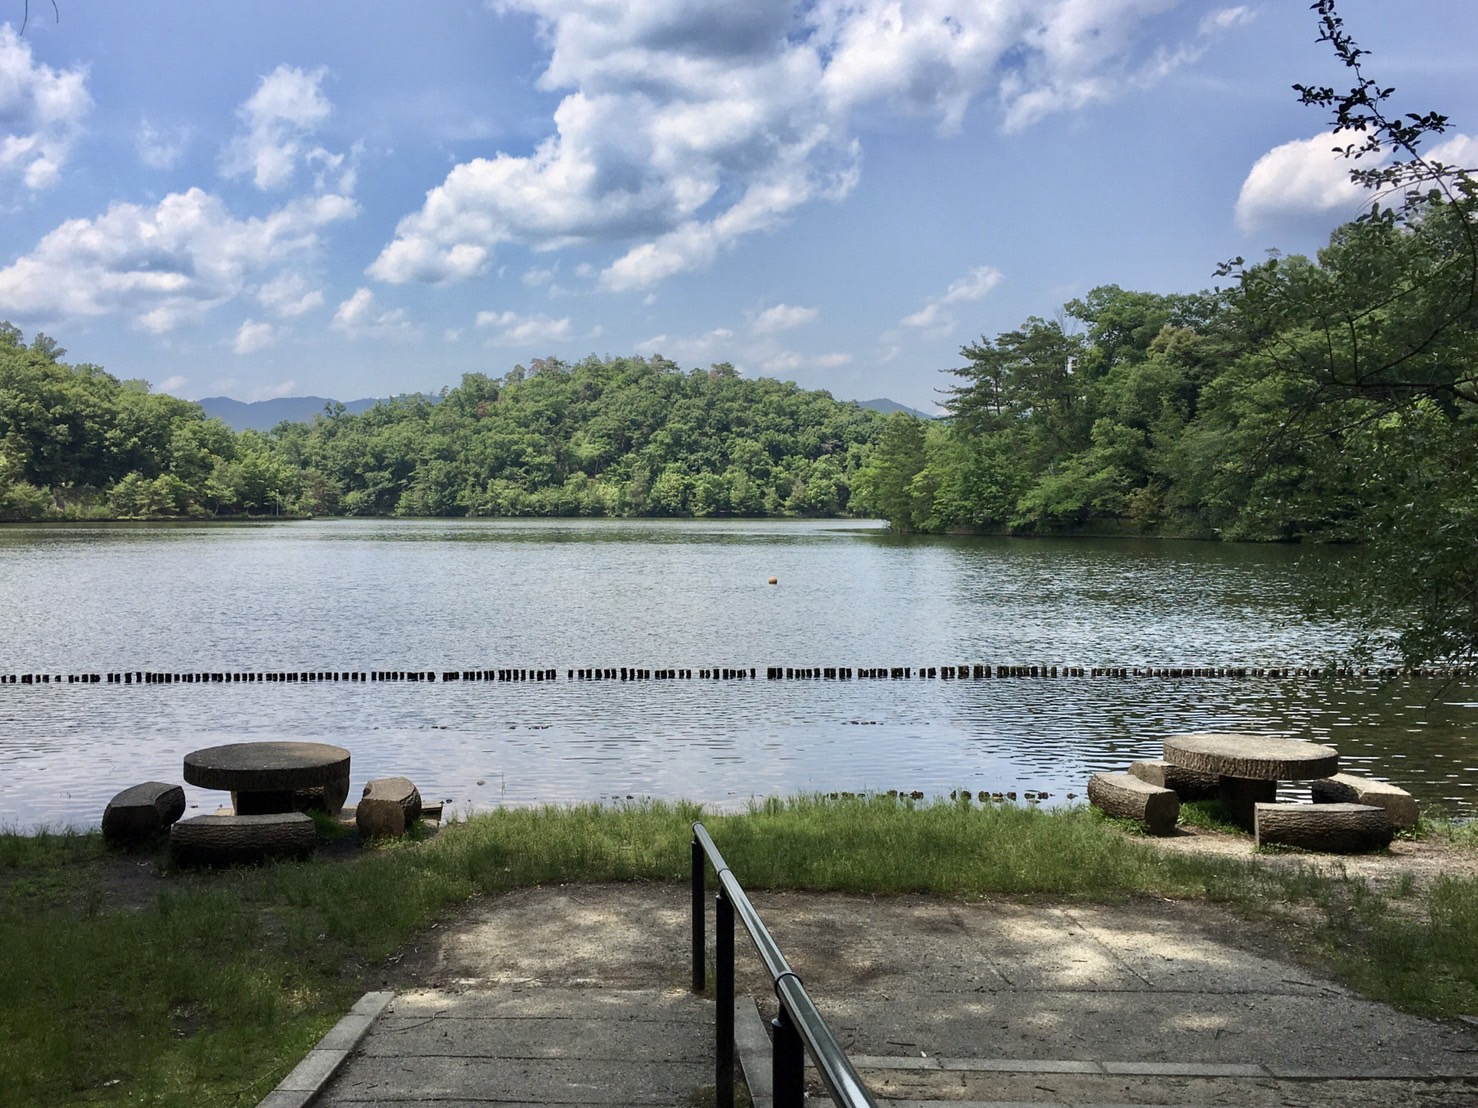
\includegraphics[width=4.8cm]{gazo/takaragaike.jpg}
\end{wrapfigure}

下鴨のさらに北あたりにある人工池とその周りの公園。ちょっとイライラしたときとかぼーっとしたいとき、とくに平日の昼間に途中でパン屋さんに寄ってから行くのがおすすめ。人が少なくて本当にぼーっとできる。ボートとか乗ってる人がいたりするとちょっとフィンランド感もある。最後に結構な坂を上らないとたどり着けないような場所にあって、それもまた自転車をこいでいる間は無心になれて良い。
%\zenkakuspace{200}

\subsubsection{北大路ビブレ(現イオンモール北大路)}
これもまた寮から北西に自転車で20分くらいの場所にあるショッピングモール。私がはじめて行った時点ですでに「ビブレありがとうイオンをよろしくねセール」みたいなものをやっていたけれど、個人的に好きなのでビブレと呼び続けている。ビブレの面白いところは、構造が本当にわけがわからないところ。3回くらいそこそこ全体を回っていてもまだ迷う。自分がどこにいるかが地図を見てもわからなくて、何回でもぐるぐるしてしまう。ぜひ一回行ってぐるぐるしてほしい。駐輪場が2時間を超えると有料なのが玉に瑕。

\subsection{あとがき}
ゴールデンウィークに帰省して寮に帰るとき、自分が自然に実家に対しても寮に対しても同じように「帰る」という言葉を使っていたことに気づいた。その時はまだ1か月かそこらしかたっていなかったけれど、あの部屋を、あの談話室を、自分は帰る場所だと認識していたんだなあと思った。もちろん人によって寮生活があうあわないはあるし、自分は同部屋の人にも同ブロックの人にも相当恵まれたからこそ楽しく過ごせている。でも、もしこれを手に取って読んでくれたあなたなら、一回くらい住んでみてもいいんじゃない?

\tatespace
最後に、
\subsection{受験と浪人について}
受験勉強は頑張ったほうがいいに決まっているし浪人もしないに越したことはない。予備校代高いし。でも頑張れないときもあるにきまってるし頑張ってもダメな時もあるじゃん。

そもそも高校生、受験生は大学生から見て相当偉い。なんか今日ちょっとさぼっちゃったなーって思ったその一日ですら、今の自分から見たらめちゃくちゃ頑張っている。そう、あなたはちゃんと頑張っているし頑張ったし、偉いし、すごいのですよ、実は。だからあんまり思いつめずに追い込み過ぎずに、あなたのために勉強してほしい。現状の充実なくして未来の充実は作れない。報われるためだけに努力するのはきっとしんどい。と、個人的には思うので。

ちなみに散歩とランニングは本当におすすめです。ちょっとすっきりするし外に出て日光を浴びるとちょっとポジティブになれる気がする。

そしてもし不合格で浪人することになったら、浪人中も思うようにいかないことはたくさんあると思います。たぶんみんなそうですが。浪人後、充実したいい時間だったなあと思えればもちろんいいし、現役の人とかをみてやっぱりちょっと無駄だったかなあと思っても、それはそれでいいんじゃないかと思います。無駄な時間があったということの意味はきっとその時間が無駄だったことそれ自体にあると思うから。

また、もし不合格で浪人以外の選択肢を選ぶことにしたら、どんなことがあるか私にはわかりませんが、それでもその選択は正解です。その時は妥協だのなんだのそんなこと思えないかもしれませんが、あなたがこれから正解にします。だからその選択は正解です。

自信をもって。

あなたが後悔なく受験を終えられますように。
